%----------------------------------------------------------------------
\section{Campaña para el paper (F6): sensibilidad, 50 realizaciones y optimalidad en lazo cerrado}\label{sec:f6}
%----------------------------------------------------------------------
\paragraph{Qué se quería saber.} Los resultados de la sección~\ref{sec:f5b} usaban entre 4 y 14
realizaciones en varias tablas y dependían de supuestos que no fijamos nosotros: la aceleración
de las reparaciones del ACS, su capacidad y la probabilidad de cada severidad de falla. Para un
paper hacían falta tres cosas: (i) saber cuáles de esos supuestos cambian las conclusiones;
(ii) repetir las tablas principales con 50 realizaciones; y (iii) medir, en lazo cerrado y con
las métricas de control de la tesis, cuán lejos del óptimo deciden N1, N2 y N3.

\paragraph{Cómo se hizo.} Se corrieron 5850 lazos cerrados en la máquina Olab (24 procesos en
paralelo, 175~min, 0 errores; \code{julia/f6\_campaign.jl}, \code{julia/F6Tasks.jl}). Las seis
campañas fueron:
\begin{itemize}
  \item \code{sens}: aceleración de las reparaciones $\mu\times\{3\cdot10^3,10^4,3\cdot10^4\}$ por capacidad
        de 30, 35, 40, 45 y 50~kg/s;
  \item \code{form}: todas las formulaciones de riesgo;
  \item \code{eta}: cuatro vectores de probabilidades de severidad;
  \item \code{det}, \code{nom} y \code{ext}: lazo cerrado con fallas del DET, familia nominal (el escenario
        de la tesis) y familia extrema, con las métricas de la tesis y una auditoría de
        optimalidad.
\end{itemize}
El riesgo se mide con el estimador de Rao--Blackwell (§8.16 del plan). En una misma corrida
puede evaluarse para varios $\mu$, porque la trayectoria de un controlador que no usa el modelo
de fallas no depende de $\mu$. Las comparaciones usan números aleatorios comunes. Tablas
completas: \code{results/f6\_paper/summary.md} (\code{python/f6\_summary.py}); figuras:
\code{python/make\_f6\_figures.py}.

\subsection{Conclusión 1: la capa de riesgo sólo sirve en un régimen, y $\mu$ lo decide}

\begin{figure}[H]\centering
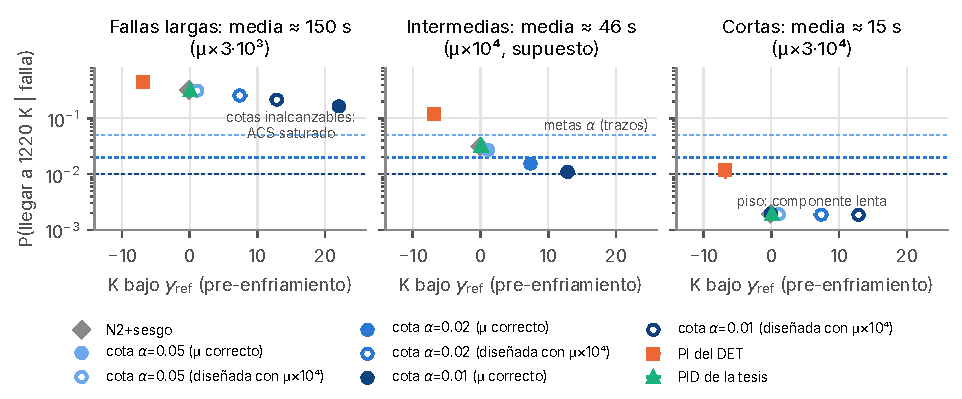
\includegraphics[width=\linewidth]{figures/fig_f6_regimes.pdf}
\caption{Riesgo frente a pre-enfriamiento a 40~kg/s, 50 realizaciones, para tres duraciones
medias de la falla. Puntos llenos: la cota diseñada con el $\mu$ verdadero. Puntos huecos: la cota
diseñada con $\mu\times10^4$ (error de especificación). Trazos: la meta $\alpha$ de cada cota.
Sólo en el panel central las cotas actúan y cumplen su meta.}
\end{figure}

La duración media de la falla se compara con el tiempo que tarda la PCT en llegar a 1220~K con
el ACS apagado ($\tau\approx165$~s). Hay tres regímenes:
\begin{itemize}
  \item \textbf{Fallas largas} (media $\approx150$~s $\approx\tau$). Para cumplir $\alpha$ habría que bajar
        la PCT a $U_\alpha\approx920$--1070~K. Es imposible: el ACS se satura, pre-enfría 22~K
        (+42\,\% de masa) y el riesgo baja de 0.32 a 0.16, todavía muy lejos de $\alpha$.
  \item \textbf{Fallas intermedias} (media $\approx46$~s, el supuesto). Es el único régimen donde
        la cota actúa y cumple su meta: 0.027 con $\alpha=0.05$ y 0.0155 con $\alpha=0.02$. Con
        $\alpha=0.01$ queda en el límite (0.0110 a 40~kg/s; 0.0138 a 30~kg/s, porque en la fase
        aguda la cota no se puede cumplir).
  \item \textbf{Fallas cortas} (media $\approx15$~s). $U_\alpha\ge1200$~K, por encima de la consigna,
        así que la cota nunca actúa. El riesgo es el piso de la componente con reparaciones de
        horas (0.0019) y ningún controlador lo baja.
\end{itemize}
El error de especificación tampoco es simétrico. Una cota diseñada para fallas de 46~s que
enfrenta fallas más cortas sobra, pero no cuesta nada (queda inactiva). Si enfrenta fallas más
largas, el riesgo sube a 0.26 con $\alpha=0.02$ y pierde la garantía. Por eso la aceleración de las
tasas es el supuesto que más hay que confirmar con el equipo.

\subsection{Conclusión 2: la capacidad y la severidad no cambian las conclusiones}
\begin{itemize}
  \item \textbf{Capacidad del ACS (30--50~kg/s).} N2 queda en 0.031 en todas las capacidades y la
        cota con $\alpha=0.02$ en 0.0147--0.0174, con 6.6--7.7~K de pre-enfriamiento. Durante una
        falla el caudal es cero sea cual sea la capacidad, así que es la duración la que fija el
        riesgo.
  \item \textbf{Probabilidades de severidad.} Con los cuatro vectores, el riesgo de N2 es
        $p_0\times0.031$ con tres cifras (figura~\ref{fig:f6-frontier}, derecha). Las fallas
        parciales no aportan riesgo medible: es el caso $\varepsilon\approx0$ de la
        Proposición~\ref{prop:eta}. La cota que conoce $\eta$ ($\alpha=0.01$) cumple su nivel con
        todos los vectores. El CVaR y la pérdida esperada con escenarios dentro del horizonte
        siguen sin actuar.
\end{itemize}

\subsection{Conclusión 3: una sola frontera, ahora con 50 realizaciones}

\begin{figure}[H]\centering
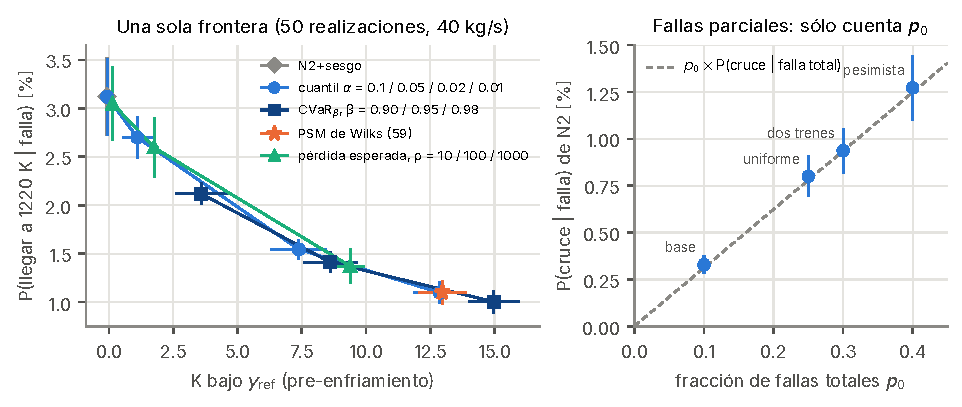
\includegraphics[width=\linewidth]{figures/fig_f6_frontier.pdf}
\caption{Izquierda: las cuatro familias de formulaciones (cuantil, CVaR, Wilks, pérdida
esperada) sobre la misma curva riesgo--pre-enfriamiento; barras: IC al 95~por ciento. Derecha:
riesgo de N2 con fallas parciales para cuatro vectores de severidad; cae sobre la recta
$p_0\times P(\text{cruce}\mid\text{falla total})$.}\label{fig:f6-frontier}
\end{figure}

Con 50 realizaciones (antes 7), las formulaciones caen sobre una sola curva, como predice la
Proposición~\ref{prop:margen}. Por ejemplo, Wilks 59 y el cuantil con $\alpha=0.01$ dan el
mismo riesgo (0.0110) con el mismo pre-enfriamiento (13.0 y 12.9~K). Lo mismo pasa con el
CVaR$_{0.95}$, la pérdida esperada con $\rho=1000$ y el cuantil con $\alpha=0.02$: 0.014--0.016 con
7.4--9.4~K. Elegir una formulación es elegir cómo se parametriza el margen, no cuánto riesgo se
compra por kelvin.

\subsection{Conclusión 4: N2 gana al PID y al PI en todas las métricas de la tesis}

\begin{table}[H]\centering\small
\begin{tabularx}{\linewidth}{@{}Y c r c r r r@{}}\toprule
Controlador (fallas del DET, 40~kg/s) & 1220~K & IAE [K\,s] & Se asienta & VT [kg/s] & DSM mín. & PCT pico\\\midrule
N1 = N2 = N3 (+sesgo) & 0/50 & $475\pm220$ & 60\,\% & 136 & 54.9~K & 1189~K\\
N2 + DSM de la tesis ($\lambda=10^4$) & 0/50 & 475 & 60\,\% & 138 & 54.9~K & 1189~K\\
N2 + cota $\alpha=0.02$ & 0/50 & $1689\pm210$ & 0\,\% & 1483 & 59.3~K & 1185~K\\
N2 + CVaR$_{0.95}$ / Wilks 59 & 0/50 & 1926 / 2806 & 2 / 0\,\% & 1454 / 1711 & 59.7 / 60.6~K & 1184 / 1183~K\\
PID de la tesis & 1/50 & $1185\pm150$ & 2\,\% & 35\,650 & 52.1~K & 1192~K\\
PI del DET & 7/50 & $3293\pm170$ & 0\,\% & 63 & 34.8~K & 1209~K\\\bottomrule
\end{tabularx}
\caption{Métricas de la tesis (Tabla~10 del paper de control) en 50 realizaciones con fallas
del DET. ``Se asienta'': fracción que entra y queda en la banda de 0.30~K. VT: variación total
del caudal mandado. DSM mín.: margen mínimo a 1244~K. Las capas de riesgo suben el IAE porque
trabajan bajo la consigna a propósito: es el precio del margen, no un defecto de seguimiento.}
\end{table}

En la familia nominal (el escenario de la tesis), N1, N2 y N3 se asientan en las 50
realizaciones: en 13~s con la bomba archivada (IAE 14.7~K\,s) y en 5.5~s a 40~kg/s (IAE
7.6~K\,s). El PID de la tesis nunca se asienta (IAE 93 y 208~K\,s) y el PI del DET tampoco (221~K\,s).
En la familia extrema con actuador físico, N2 no llega a 1220~K en ninguna realización (IAE
919~K\,s), frente a 3654~K\,s del PID y 5755~K\,s del PI. Con la bomba archivada, en cambio, llega
en 22 de 50, porque la capacidad no alcanza (sección~\ref{sec:extremos}).

\subsection{Conclusión 5: en lazo cerrado, N3 y N2 deciden prácticamente en el óptimo}

En 3150 consultas de lazo cerrado (cada 10 o 20 consultas, en las tres familias) se comparó la
decisión del lazo con N1, N2, N3 pulido y N3 desde un arranque en frío, todos con el mismo
costo P0 sobre el ROM.
\begin{itemize}
  \item \textbf{Cómo medir la brecha.} En el 53--85\,\% de las consultas el seguimiento es
        exacto y el mejor costo es $J_{\rm best}\approx10^{-12}$. Ahí la brecha relativa
        $J/J_{\rm best}-1$ no significa nada (la primera tabla daba $10^5$\,\%). Se usa el exceso
        en error RMS sobre el horizonte, $\sqrt{J/K}-\sqrt{J_{\rm best}/K}$.
  \item \textbf{Resultado.} N3 queda a $\le2.5\cdot10^{-8}$~K del mejor. N2 queda a
        $\le6\cdot10^{-4}$~K (brecha relativa $\le0.03$\,\% donde $J_{\rm best}\ge1$~K$^2$).
        N1 queda a $\le7\cdot10^{-4}$~K, salvo en la familia extrema con actuador físico: hasta
        0.33~K (6\,\%), porque linealiza una sola vez y las jugadas son grandes.
  \item \textbf{Ningún óptimo mejor.} El arranque en frío de N3 no encontró nada mejor en
        ninguna consulta.
\end{itemize}
Es evidencia de optimalidad local con varios arranques en 3150 consultas, no un certificado
global (que sigue limitado a las dos consultas de F3c).

\takeaway{Con 50 realizaciones, cinco capacidades y cuatro modelos de severidad, las
conclusiones se sostienen: una sola frontera riesgo--pre-enfriamiento, una garantía calibrada
($P\le\alpha$), y N2 en el óptimo y en tiempo real, mejor que el PID y el PI en todas las métricas
de la tesis. La condición de aplicabilidad es la aceleración de las reparaciones. La capa de
riesgo sólo actúa si las fallas duran, en promedio, algo menos que el tiempo hasta 1220~K. Si
duran mucho menos, sobra; si duran tanto como ese tiempo, ningún controlador cumple $\alpha$.}
